% Beamer slide template prepared by Tom Clark <tom.clark@op.ac.nz>
% Otago Polytechnic
% Dec 2012

\documentclass[10pt]{beamer}
\usetheme{Dunedin}
\usepackage{graphicx}
\usepackage{fancyvrb}

\newcommand\codeHighlight[1]{\textcolor[rgb]{1,0,0}{\textbf{#1}}}

\title{Factory Patterns}

\author[IN710]{Object Oriented System Design}
\institute[Otago Polytechnic]{
  Otago Polytechnic \\
  Dunedin, New Zealand \\
}
\date{}
\begin{document}

%----------- titlepage ----------------------------------------------%
\begin{frame}[plain]
  \titlepage
\end{frame}

\begin{frame}
	\frametitle{Disclaimer}

	I hate factory patterns.
\end{frame}

\begin{frame}
	\frametitle{Partial retraction}

	I used to hate factory patterns because I saw them 
	used pointlessly by ``enterprise'' programmers who
	slavishly used patterns without thinking.

	This led to code that was hard to read and hard to reason about.
\end{frame}

\begin{frame}
	\frametitle{Patterns are just tools}

	Our goal is always to write readable good code.  Patterns 
	are just a tool you can use when it helps with this goal.
\end{frame}

\begin{frame}
	\frametitle{Problem 0}

	\begin{itemize}
		\item You're writing a game.
		\item In your game players fight zombies, vampires, and skeletons.
		\item At some point in the game you want to generate
			some monsters, but you don't know which type until
			runtime.
	\end{itemize}
\end{frame}

\begin{frame}
	\frametitle{Problem 1}
	\begin{itemize}
		\item You're writing a document layout module.
		\item Your module includes a family of layout
			classes for various page dimensions (e.g.,
			broadsheet, tabloid, poster board)
		\item Users will select which layout type to use
			at runtime.
	\end{itemize}
\end{frame}

\begin{frame}
	\frametitle{The problem, simply}

	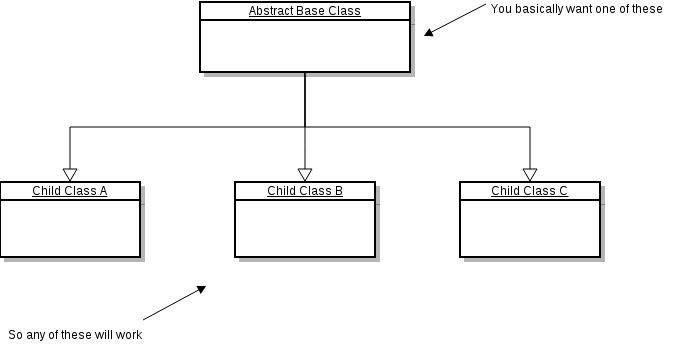
\includegraphics[width=100mm]{basic_uml.png}
\end{frame}

\begin{frame}[fragile]
	\frametitle{Solution: build a factory}

	\begin{verbatim}

	class MonsterFactory:
            
            def create_monster(desired_type):
                if desired_type == 'vampire':
                    return Vampire()
                elif desired_type == 'zombie':
                    return Zombie()
                elif desired_type == 'skeleton':
                    return Skeleton()
                else:
                    return None
        \end{verbatim}
\end{frame}

\begin{frame}
	\frametitle{Is that it?}

	\begin{itemize}
		\item Sort of, yes.
		\item Ok, not really.
		\item We can implement various types of
			decision-making logic in our factories.
		\item Maybe we need to do a bit of housekeeping
			before we create a \texttt{Monster}.
		\item Maybe we need to create a parallel object
			at the same time we create a \texttt{Monster},
			e.g., a \texttt{MonsterRenderer}.
	\end{itemize}
\end{frame}

\begin{frame}
	\frametitle{Exercise}

	\begin{itemize}
            \item Suppose we have data records in dictionaries
		    with strings as keys.
	    \item We want to represent these records as different
		    sorts of documents:
		    \begin{enumerate}
			    \item JSON
			    \item YAML
			    \item XML
		    \end{enumerate}
	    \item Write a set of Document classes, e.g.,
		    \texttt{JSONDocument} that implement a method,
		    \texttt{dump()} that emits a data record in the 
		    correct document format.
	    \item Then, write a \texttt{DocumentFactory} class that
		    produces the desired type of document class.
	    \item Experiment with different types of creation logic by
		    implementing different create methods.
	    \item Tips:
		    \begin{enumerate}
			    \item Look for libraries to help you.
			    \item Don't go nuts on the XML. If you 
				    can produce a crude XML structure
				    that suffices.
		    \end{enumerate}
	\end{itemize}

\end{frame}



\end{document}
